\newvideofile{asynchronmaschine}{Asynchronmaschine}
\v{
	\begin{frame}{Lernziele}
		\begin{Lernziele}{Asynchronmaschine}
			Du kannst
			\begin{itemize}
				\item den grundlegenden Aufbau und die Hauptbauteile einer Asynchronmaschine beschreiben.
				\item den Schlupf definieren und seine Auswirkung auf Drehzahl und Betrieb erklären.
				\item Drehmoment‑Schlupf‑Verhalten qualitativ beschreiben und wichtige Kennwerte wie Anlauf-, Nenn- und Kippmoment zuordnen.
			\end{itemize}
		\end{Lernziele}
		\speech{LernzieleAsynchronmaschine}{1}{Nachdem wir die Synchronmaschine betrachtet haben, wollen wir nun einen Blick auf die Asynchronmaschine werfen, welche in Gegenüberstellung zur Synchronmaschine eine wesentlich einfachere Technik zur Regelung benötigt.}
		\silence{2}
	\end{frame}
}
\section{Asynchronmaschine}
\s{Die Asynchronmaschine ist ebenfalls eine Drehfeldmaschine. Der Stator ist identisch zum Stator der Synchronmaschine, der Rotor ist hingegen in der häufigsten Version dieses Maschinentyps, beim sogenannten Käfigläufer, passiv.}
\begin{frame}\ftx{Asynchronmaschine Aufbau}\index{Asynchronmaschine>Aufbau}\s{\subsection{Aufbau}}
	\fo{width=0.65\textwidth, alt={Schematische Schnittansicht einer Käfigläufer-Asynchronmaschine. Das Bild zeigt die verschiedenen Komponenten des Motors, einschließlich des Gehäuses mit Blechpaket und den darin befindlichen Drehstromwicklungen. Außerdem ist der Läuferkäfig zu sehen, der mit Blechpaketen bestückt ist, sowie am hinteren Ende die Lüfterflügel, die von einer Flügelhaube abgedeckt werden.}}{height=0.9\textheight}{Aufbau_Asynchron_Kaefig1}{
		\onslide<2->{\put(79,0){\line(-1,1){29.5}}\put(79.2,0){Gehäuse mit Blechpaket}
		\put(79,6){\line(-1,1){27}}\put(79.3,6){Drehstromwicklung}
		\put(90,12){\line(-1,1){40}}\put(90.3,12){Läuferkäfig}
		\put(90,18){\line(-1,1){32}}\put(90.3,18){Blechpaket}
		\put(103,36){\line(-1,1){10}}\put(103.3,36){Flügelhaube}
		\put(103,42){\line(-1,1){27}}\put(103.3,42){Lüfterflügel}}

	}{{\bf Aufbau einer Käfigläufer-Asynchronmaschine.} Die Bleche des Rotorzylinders wurden der Anschaulichkeit halber zur Hälfte beschnitten, um den Käfig freizulegen.}
	
	\speech{AufbauASM}{1}{Die Asynchronmaschine ist wie die Synchronmaschine eine sogenannte Drehfeld-maschine. Der Stator ist identisch zum Stator der Synchronmaschine, der Rotor ist hingegen in der häufigsten Version dieses Maschinen-typs – dem Käfigläufer – passiv.}
	\silence{2}
	\speech{AufbauASM}{2}{Der Rotor besteht aus einem zylindrischen Blechpaket, das mit Kurzschlussstäben, dem sogenannten Läuferkäfig, versehen ist. Der Stator verfügt über die selbe Drehstromwicklung wie die Synchronmaschine. Diese ist hier in orange dargestellt. Das Gehäuse hat in den meisten Fällen ein angebautes Lüfterrad, das mit der gleichen Drehzahl der Maschine dreht und dafür sorgt, dass die Maschine während des Betriebs gekühlt wird.}
	\silence{2}
\end{frame}

\begin{frame}\ftb{\index{Käfigläufer}Käfigläufer}
	\begin{itemize}
		\item In den Nuten des Läuferblechpaketes liegen leitfähige Stäbe.
		\item Stirnseitig sind die Stäbe durch Kurzschlussringe miteinander verbunden.
		\item Zusammen bilden diese Komponenten einen Käfig (ähnlich Hamsterkäfig).
		\item Stäbe werden geschrägt ausgeführt zur Reduktion von Oberwellen im umlaufenden magnetischen Feld.
	\end{itemize}
		\f{width=0.5\textwidth, alt={Schematische Darstellung eines Kupferzylinders, dessen ringförmige Vorder- und Rückseite mit Lamellen verbunden sind. Die Lücken zwischen den Lammellen sind mit Blechpaketen gefüllt.}}{height=0.6\textheight}{Aufbau_Asynchron_Kaefig2}{{\bf Käfig eines Asynchronrotors.} Zur Hälfte mit Blechpaket gezeigt.}
		\speech{ASMKaefiglaufer}{1}{Der Käfigläufer ist die gängigste Bauform einer Asynchronmaschine. Der Läufer besteht aus einem Läuferblechpaket, in dessen Nuten leitfähige Stäbe eingelegt sind. Diese Stäbe ragen über die Stirnseiten hinaus und werden dort durch sogenannte Kurzschlussringe miteinander verbunden, sodass ein geschlossener elektrischer Stromweg entsteht. Durch die Anordnung der Stäbe und Ringe bildet sich ein käfigähnliches Gebilde, das den Namen prägt. Wenn das am Stator erzeugte, umlaufende Magnetfeld den Läufer durchsetzt, werden in den Stäben Ströme induziert. Diese Ströme erzeugen wiederum ein eigenes Magnetfeld, das mit dem Statorfeld wechselwirkt und so ein Drehmoment auf den Läufer ausübt. Die Stäbe sind häufig schräg ausgeführt (keilförmig oder geneigt angeordnet), um die unerwünschten Oberwellen im umlaufenden Magnetfeld zu reduzieren. Dadurch verbessert sich das Anlaufverhalten und die Laufruhigkeit der Maschine.}
	\silence{2}
\end{frame}


\begin{frame}	\ftb{Anlauf der ASM}\index{Asynchronmaschine>Anlauf}
	\onslide<2->{
		\begin{itemize}
			\item Der Stator erzeugt im Ständer eine umlaufende magnetische Wanderwelle mit der Winkelgeschwindigkeit:
			      $\omega_\mathrm{s} = \frac{\omega_0}{p}$.
			\onslide<3->{\item Auf den ruhenden Läufer wirkt ein zeitlich veränderliches Feld mit der Frequenz $\omega_\mathrm{s}$.}
			\onslide<4->{\item Das magnetische Drehfeld durchsetzt den Läufer und induziert eine Spannung mit der Frequenz $\omega_\mathrm{s}$.}
			\onslide<5->{\item Aus der Spannungsinduktion resultiert ein Stromfluss, da die Läuferwicklungen kurzgeschlossen sind.}
			\onslide<6->{\item Der induzierte Rotorstrom wirkt der auf ihn einwirkenden Änderung des Statorfeldes entgegen (Lenzsche Regel).}
			\onslide<7->{\item Statorfeld und Rotorstrom wechselwirken durch die Lorentzkraft – es kommt zur Ausbildung eins Drehmoments.}
			\onslide<8->{\item Das Drehmoment wirkt in Richtung des Ständerdrehfelds.}
			\onslide<9->{\item Der Läufer beginnt sich zu drehen.}
		\end{itemize}
	}
	\speech{ASMAnlauf}{1}{Beim Anlauf einer Asynchronmaschine treffen mehrere Effekte zusammen, die nur im dynamischen Übergang – also vom Stillstand zum Drehzahl-gleichgewicht – relevant sind. Sehen wir uns nun einmal schrittweise an, wie der Anlauf einer Asynchronmaschine aussieht.}
	\silence{2}
	\speech{ASMAnlauf}{2}{Der Stator erzeugt im Ständer eine umlaufende magnetische Wanderwelle mit der Winkelgeschwindigkeit Omega S. Diese Winkelgeschwindigkeit ist der Quotient aus der Netzwinkelgeschwindigkeit Omega Null und der Pohlpaarzahl P.}
	\speech{ASMAnlauf}{3}{Auf den noch ruhenden Läufer wirkt ein zeitlich veränderliches Feld mit der Frequenz der Winkelgeschwindigkeit.}
	\speech{ASMAnlauf}{4}{Das magnetische Drehfeld durchsetzt den Läufer und induziert eine Spannung mit der Frequenz der Winkelgeschwindigkeit.}
	\speech{ASMAnlauf}{5}{Aus der Spannungsinduktion resultiert ein Stromfluss, da die Läuferwicklungen kurzgeschlossen sind.}
	\speech{ASMAnlauf}{6}{Der induzierte Rotorstrom wirkt entsprechend der Lenzschen Regel entgegen der auf ihn einwirkenden Änderung des Statorfeldes.}
	\speech{ASMAnlauf}{7}{Statorfeld und Rotorstrom wechselwirken durch die Lorentz-Kraft aufeinander, wodurch ein Drehmoment entsteht.}
	\speech{ASMAnlauf}{8}{Das Drehmoment wirkt dabei in Richtung des Ständerdrehfelds.}
	\speech{ASMAnlauf}{9}{Und der Läufer beginnt schließlich sich zu drehen.}
	\silence{2}
\end{frame}

\begin{frame}	\ftb{Betrieb der ASM}    \index{Asynchronmaschine>Funktionsprinzip}
	\onslide<2->{
	\begin{itemize}
		\item Mit steigender Drehzahl des Läufers nimmt die Wirkung des Statorfeldes ab:
		$\omega_\mathrm{r} = \omega_\mathrm{s} - \omega_\mathrm{mech}$.
		\onslide<3->{\item Mit steigender Drehzahl sinken sowohl der Betrag als auch die Frequenz der induzierten Spannung im Rotor.}
		\onslide<3->{\item Der Betrag des Drehmoments sinkt.}
		\onslide<4->{\item Drehen sich der Läufer und Statorfeldes mit der gleichen Frequenz, ist die synchrone Drehzahl erreicht.}
		\onslide<5->{\item Die Läuferwicklungen werden nicht vom Statorfeld beeinflusst.}
		\onslide<6->{\item Induzierter Strom und Drehmoment der Maschine werden zu Null.}
		\onslide<7->{\item Durch Reibungseffekte wird der Rotor wieder abgebremst – es kommt zur erneuten Ausbildung eines Drehmoments.}
		\onslide<8->{\item Im Gleichgewichtszustand stellt sich eine Drehzahl knapp unter der synchronen Drehzahl ein.}
	\end{itemize}
	}
	\speech{ASMBetrieb}{1}{Schauen wir uns ergänzend dazu den Betrieb einer Asynchronmaschine schrittweise an.}
	\silence{2}
	\speech{ASMBetrieb}{2}{Die Relativdrehzahl Omega R, auch Schlupffrequenz genannt, gegenüber der des Statorfeldes Omega S entspricht der Drehzahl des Statorfeldes abzüglich der mechanischen Drehzahl des Läufers. Mit steigender Drehzahl des Läufers nimmt also die Wirkung des Statorfeldes ab.}
	\speech{ASMBetrieb}{3}{Mit steigender Drehzahl sinken außerdem sowohl der Betrag als auch die Frequenz der induzierten Spannung im Rotor.}
	\speech{ASMBetrieb}{4}{Die Synchrone Drehzahl ist dann erreicht, wenn sich der Läufer und das Statorfeld mit der selben Frequenz drehen.}
	\speech{ASMBetrieb}{5}{Die Läuferwicklungen werden dann nicht mehr vom Statorfeld beeinflusst.}
	\speech{ASMBetrieb}{6}{Der induzierte Strom und der Drehmoment der Maschine gehen an dieser Stelle zu Null.}
	\speech{ASMBetrieb}{7}{Allerdings bremsen Reibungseffekte den Rotor kontinuierlich, sodass es dadurch erneut zu einer Drehmomentwirkung auf den Rotor kommt.}
	\silence{2}
	\speech{ASMBetrieb}{8}{Schließlich stellt sich ein Gleichgewichts-zustand ein. Dieser liegt knapp unter der synchronen Drehzahl.}
	\silence{2}
\end{frame}


\begin{frame}\ftb{Drehzahl/Drehmomenten-Kennlinie}
	\begin{columns}
		\column[c]{0.3\textwidth}
			\b{Schlupf:}
			\s{Die Drehzahl/Drehmomenten-Kennlinie ist bei der Asynchronmaschine nichtlinear und kann in mehrere Abschnitte unterteilt werden. Häufig wird die Kennlinie wie in Abbildung \ref{kloss} gezeigt über den Schlupf $s$ aufgetragen. Der Schlupf\index{Schlupf} bezeichnet die prozentuale Abweichung der mechanischen Drehgeschwindigkeit des Rotors $n_\mathrm{r}$ von der elektrischen Drehgeschwindigkeit $n_\mathrm{s}$ des speisenden Netzes im Stator.}
			\nomenclature[F]{$s$}{Schlupf der Asynchronmaschine}
			\nomenclature[F]{$\omega_\mathrm{s}$}{Synchrone Drehfrequenz des speisenden Netzes \nomunit{$\frac{1}{\mathrm{s}}$}}
			\nomenclature[F]{$\omega_\mathrm{r}$}{Drehfrequenz des Rotors \nomunit{$\frac{1}{\mathrm{s}}$}}
			\begin{eq}
				s = \frac{\omega_\mathrm{s} - \omega_\mathrm{r}}{\omega_\mathrm{s}}
			\end{eq}

			\s{Ein Schlupf von $s=1$ ($100\%$) entspricht daher dem Stillstand der Maschine oder Drehzahl $n=0$, ein Schlupf von $s=0$ entspricht dem netzsynchronen Betrieb, der jedoch bei der Asynchronmaschine niemals auftreten kann, da das Drehmoment in dem Fall Null wird.}

			\uncover<2->{
				\s{Die Drehzahl/Drehmomenten-Kennlinie wird auch als Klosssche Kennlinie bezeichnet und kann durch die Gleichung \ref{GlKloss} ausgedrückt werden:}
				\b{Klosssche Gleichung}
				\begin{eq}
					M = \frac{2\cdot M_\mathrm{K}}{\frac{s_\mathrm{K}}{s} + \frac{s}{s_\mathrm{K}}}\label{GlKloss}
				\end{eq}
				\nomenclature[F]{$s_\mathrm{K}$}{Kippschlupf der Asynchronmaschine}
				\nomenclature[F]{$M_\mathrm{K}$}{Kippmoment der Asynchronmaschine \nomunit{Nm}}
			}
			\uncover<3>{

				\s{Der Schlupf entspricht bei großen Maschinen in sehr guter Näherung den prozentualen Verlusten der Maschine:}
				\b{Schlupf entspricht den prozentualen Verlusten:}
				\begin{eq}
					\eta \approx 1-s
				\end{eq}
			}
		\column[c]{0.7\textwidth}
		\s{
			\fu{
				\input{Tikz/src/klosssche_kennlinie.tex}\alttext{Diagramm, das den Zusammenhang aus Drehzahl und Drehmoment einer Asynchronmaschine zeigt. Die Drehzahl wird auf der X-Achse abgebildet von S (links) bis Minus S (rechts), während das Drehmoment auf der Y-Achse dargestellt wird. Innerhalb des Diagramms befindet sich eine Kurve, die die Drehzahl/Drehmomenten-Kennlinie zeigt. Sie bewegt sich langsam steigend im positiven Bereich von S von der linken Seite des Diagramms immer steiler werdend, bis sie kurz vor dem Nullpunkt ein Maximum am Punkt SK erreicht und genau zum Nullpunkt hin steil abfällt. Auf der negativen Seite von S des Diagramms verhält sich die Kurve äquivalent, jedoch über die Y-Achse gespiegelt. Links befindet sich der Bereich, an dem die Asynchronmaschine als Bremse fungiert, bis zum Punkt des Stillstands, an dem s = 1 ist. In dem rechts davon folgenden Bereich agiert die Asynchronmaschine als Motor bis zum Maximum SK. Auf der negativen Seite von S wirkt die Asynchronmaschine ab dem Minimum Minus SK als Generator. Das Diagramm zeigt, dass sich die Asynchronmaschine untersynchron verhält, wenn S > 0 ist, und übersynchron, wenn S < 0 ist.}
				}{{\bf Klossche Kennlinie.} Drehzahl/Drehmomenten-Kennlinie einer Asynchronmaschine. \label{kloss}}
		}
		\b{
			\fu{
				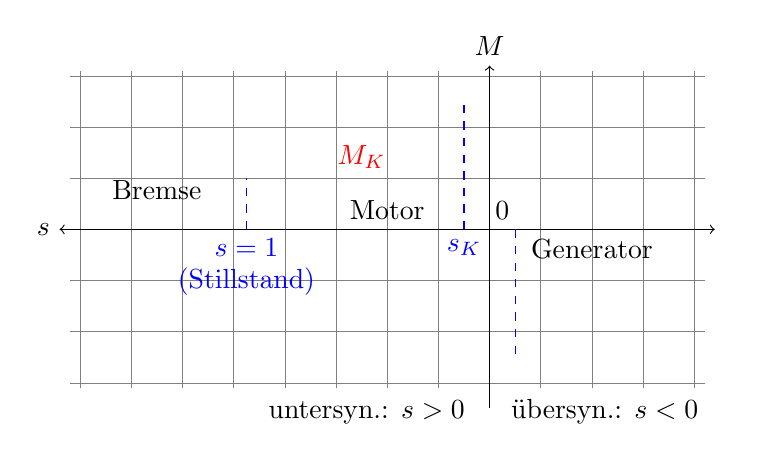
\begin{tikzpicture}[domain=-16:8, samples=200,  scale=0.65]
				\draw[very thin,color=gray] (-8.2,-3.1) grid (4.2,3.1);
				\draw[<->] (-8.4,0) node[left] {$s$} -- (4.4,0) node[right] {$\varPhi$};
				\draw[->] (0,-3.5) -- (0,3.2) node[above] {$M$};
				\draw[color=red, scale=1/2, smooth] plot[id=klossche_kennlinie] function{-5 * (2 / (x / 0.96 + 0.96 / x))} node[right] {};
				\draw (0.25,0) node[above] {$0$};
				\draw[color=red] (-2.5,1) node[above] {$M_K$};
				\draw[dashed, color=blue] (-0.5,0) node[below] {${s_K}$} -- (-0.5,2.5);
				\draw[dashed, color=blue] (0.5,0) node[above] {} -- (0.5,-2.5);
				\draw[dashed, color=blue] (-4.75,0) node[below] {${s = 1}$} -- (-4.75,1);
				\draw[color=blue] (-4.75,-0.55) node[below] {(Stillstand)};
				\draw (-6.5,0.4) node[above] {Bremse};
				\draw (-2,0) node[above] {Motor};
				\draw (2,0) node[below] {Generator};
				\draw (-2.4,-4) node[above] {untersyn.: $s > 0$};
				\draw (2.25,-4) node[above] {übersyn.: $s < 0$};
				\end{tikzpicture}
				}{Klossche Kennlinie}
		}

	\end{columns}
	\speech{ASMDrehzahlDrehmomentkennlinie}{1}{Die Drehzahl-Drehmoment-Kennlinie ist bei der Asynchronmaschine nichtlinear und kann in mehrere Abschnitte unterteilt werden. Häufig wird die Kennlinie wie sie hier dargestellt ist, über den Schlupf S aufgetragen. Der Schlupf bezeichnet die prozentuale Abweichung der mechanischen Drehgeschwindigkeit des Rotors N-R von der elektrischen Drehgeschwindigkeit N-S des speisenden Netzes im Stator.}
	\silence{2}
	\speech{ASMDrehzahlDrehmomentkennlinie}{2}{Ein Schlupf von S gleich Eins, also von Einhunddert Prozent, entspricht daher dem Stillstand der Maschine oder auch der Drehzahl von Null umdrehungen. Ein Schlupf von S gleich Null entspricht dem absolut netzsynchronen Betrieb, der jedoch bei der Asynchronmaschine in der Praxis niemals auftreten kann, da das Drehmoment in dem Fall Null wäre.}
	\silence{2}
	\speech{ASMDrehzahlDrehmomentkennlinie}{3}{Der Schlupf entspricht bei großen Maschinen in sehr guter Näherung den prozentualen Verlusten der Maschine. Der Wirkungsgrad einer Asynchronmaschine ist also Eins abzüglich des Schlupfes.}
	\silence{2}
\end{frame}


\begin{frame}\ftx{Beispiel: Asynchronmaschine}
	\begin{bsp}{Asynchronmaschine}{}
		Ein Drehstrom-Asynchronmotor hat die folgenden Typenschildangaben:
		\begin{columns}
			\column[c]{0.5\textwidth}
				\begin{itemize}
					\item Nennleistung: $10\,$kW
					\item Nenndrehzahl: $1440\,\frac{\mathrm{U}}{\mathrm{min}}$
				\end{itemize}
			\column[c]{0.5\textwidth}
				\begin{itemize}
					\item Frequenz: $50\,$Hz
					\item Kippschlupf: 25\%
				\end{itemize}
		\end{columns}\b{\vspace{0.3cm}}
		Berechnen Sie das Nennmoment, das Kippmoment und das Anlaufmoment.
		\s{
			\begin{align*}
				P_\mathrm{N} &= M_\mathrm{N}\cdot \omega_\mathrm{N} = M_\mathrm{N}\cdot 2\pi n_\mathrm{N}\\
				M_\mathrm{N} &= \frac{P_\mathrm{N}}{2\pi n_\mathrm{N}} = \frac{10\cdot 10^3\,\mathrm{W}}{2\pi\cdot 1440 \frac{1}{60\,\mathrm{s}}} = 66,31\,\mathrm{Nm}\\
				s_\mathrm{N} &= \frac{\omega_\mathrm{s} - \omega_\mathrm{r}}{\omega_\mathrm{s}}\\
				&=\frac{2\pi \cdot 1500 \,\frac{1}{60\,\mathrm{s}} - 2\pi\cdot 1440\,\frac{1}{60\,\mathrm{s}}}{2\pi \cdot 1500 \,\frac{1}{60\,\mathrm{s}}}\\
				& = 0,04
			\end{align*}
			Für die Berechnung der weiteren Momente wird Gleichung \ref{GlKloss} für die Fälle Nennbetrieb und Stillstand ausgerechnet.
			\begin{align*}
				M &= \frac{2\cdot M_\mathrm{K}}{\frac{s_\mathrm{K}}{s} + \frac{s}{s_\mathrm{K}}}\\
				M_\mathrm{K} &= \frac{M_\mathrm{N}}{2}\cdot\left(\frac{s_\mathrm{K}}{s_\mathrm{N}} + \frac{s_\mathrm{N}}{s_\mathrm{K}}\right)\\
				&= \frac{66,31\,\mathrm{Nm}}{2}\cdot\left(\!\frac{0,25}{0,04} + \frac{0,04}{0,25}\!\right) = 212,54\,\mathrm{Nm}\\
				M_\mathrm{A} &= \frac{2\cdot 212,54\,\mathrm{Nm}}{\frac{0,25}{1} + \frac{1}{0,25}} = 100,02\,\mathrm{Nm}
			\end{align*}
		}
		\b{
		\only<2-5>{
				\begin{align*}
					\onslide<2->{P_\mathrm{N} &= M_\mathrm{N}\cdot \omega_\mathrm{N} \onslide<3->{= M_\mathrm{N}\cdot 2\pi n_\mathrm{N}}}\\
					\onslide<4->{M_\mathrm{N} &= \frac{P_\mathrm{N}}{2\pi n_\mathrm{N}} \onslide<5->{= \frac{10\cdot 10^3\,\mathrm{W}}{2\pi\cdot 1440 \frac{1}{60\,\mathrm{s}}} = 66,31\,\mathrm{Nm}}}\\
				\end{align*}
		}
		\only<6-10>{
				\begin{align*}
					\onslide<6->{M &= \frac{2\cdot M_\mathrm{K}}{\frac{s_\mathrm{K}}{s} + \frac{s}{s_\mathrm{K}}}}\\
					\onslide<7->{s_\mathrm{N} &= \frac{\omega_\mathrm{s} - \omega_\mathrm{r}}{\omega_\mathrm{s}}}\\
					\onslide<8->{&=\frac{2\pi \cdot 1500 \,\frac{1}{60\,\mathrm{s}} - 2\pi\cdot 1440\,\frac{1}{60\,\mathrm{s}}}{2\pi \cdot 1500 \,\frac{1}{60\,\mathrm{s}}} = 0,04}\\
					\onslide<9->{M_\mathrm{K} &= \frac{M_\mathrm{N}}{2}\cdot\left(\frac{s_\mathrm{K}}{s_\mathrm{N}} + \frac{s_\mathrm{N}}{s_\mathrm{K}}\right)}\\
					\onslide<10->{&= \frac{66,31\,\mathrm{Nm}}{2}\cdot\left(\!\frac{0,25}{0,04} + \frac{0,04}{0,25}\!\right) = 212,54\,\mathrm{Nm}}\\
				\end{align*}
		}
		\only<11-12>{
				\begin{align*}
					\onslide<11->{M &= \frac{2\cdot M_\mathrm{K}}{\frac{s_\mathrm{K}}{s} + \frac{s}{s_\mathrm{K}}}}\\
					\onslide<12->{M_\mathrm{A} &= \frac{2\cdot 212,54\,\mathrm{Nm}}{\frac{0,25}{1} + \frac{1}{0,25}} = 100,02\,\mathrm{Nm} }
				\end{align*}
		}
		}
	\end{bsp}
	\speech{ASMDrehzahlBeispielrechnung}{1}{Sehen wir uns dazu nun noch ein Rechenbeispiel an. Gegeben ist hier ein Drehstrom-Asynchronmotor von dem die Nennleistung, die Nenndrehzahl, die Betriebs-Frequenz und der Kippschlupf bekannt sind. Berechnen wir dazu das Nennmoment M, das Kippmoment M-K und abschließend das Anlaufmoment M-A.}
	\silence{2}
	\speech{ASMDrehzahlBeispielrechnung}{2}{Die Formel zur Berechnung der Nennleistung P-N ist gleich dem Nennmoment multipliziert mit der Winkelgeschwindigkeit der Nennleistung.}
	\speech{ASMDrehzahlBeispielrechnung}{3}{Die Winkelgeschwindigkeit, die hier benötigt wird, ist nicht bekannt. Wie aber bereits im Video zur Gleichstrommaschine besprochen, ist die Winkelgeschwindikeit das Produkt aus der Drehzahl N und 2 Pi. Die Nenndrehzahl der Asynchronmaschine ist bekannt. Dass es sich hierbei um die Nenndrehzahl handelt, also die Drehzahl am Nennmoment, wird angezeigt durch den Index N. Wir können also diese Formel an der Stelle der Nenndrehzahl einsetzten.}
	\silence{2}
	\speech{ASMDrehzahlBeispielrechnung}{4}{Stellen wir nun die Formel nach der gesuchten Größe um, also dem Nennmoment M-N.}
	\speech{ASMDrehzahlBeispielrechnung}{5}{Wenn wir dann die Werte einsetzten und den Term kürzen, errechnet sich für die gegebenen Größen ein Nennmoment von 66 Komma Drei Eins Newton-Meter. Damit hätten wir den ersten gesuchten Wert der gegebenen Asynchronmaschine ermittelt.}
	\silence{4}
	\speech{ASMDrehzahlBeispielrechnung}{6}{Um im nächsten Schritt den Kippmoment zu berechnen, wenden wir die Klosssche Gleichung an, die wir zuvor im Zusammenhang mit der Drehzahl-Drehmoment-Kennlinie betrachtet haben. Da wir das Kippmonent M-K errechnen wollen, müssen wir die Gleichung nach M-K umstellen. Der Kippschlupf S-K ist bekannt. Doch um das Kippmoment berechnen zu können, fehlt uns noch eine Größe: Und zwar der Schlupf S am Nennmoment. }
	\silence{2}
	\speech{ASMDrehzahlBeispielrechnung}{7}{Berechnen wir also zunächst den Schlupf. Weil sich dieser auf das Nennmoment bezieht, bezeichnen wir ihn als Schlupf S-N. Die Formel zur Berechnung des Schlupfes haben wir vorhin an der Stelle der Drehzahl-Drehmoment-Kennlinie schon kurz angeschaut. Er ist die relative Differenz zwischen synchroner Winkelgeschwindigkeit Omega S und Rotorwinkelgeschwindigkeit Omega R.}
	\silence{2}
	\speech{ASMDrehzahlBeispielrechnung}{8}{Setzten wir nun die Werte in die Gleichung ein und kürzen, erhalten wir einen Schlupf von S-N gleich Null Komma Null Vier.}
	\silence{2}
	\speech{ASMDrehzahlBeispielrechnung}{9}{Nun haben wir alle Größen, um das Kippmoment berechnen zu können. Stellen wir also die Klossche Gleichung nach M-K um.}
	\speech{ASMDrehzahlBeispielrechnung}{10}{Das Nenmoment M-N und den Schlupf am Nennmoment haben wir eben berechnet. Der gegebene Kippschlupf von Fünfundzwanzig Prozent entspricht natürlich 0,25. Setzten wir nund die Werte in die Gleichung ein. Es ergibt sich ein Kippmoment von Zweihundertzwölf Komma Vierundfünfzig Newton-Meter.}
	\silence{4}
	\speech{ASMDrehzahlBeispielrechnung}{11}{Bleibt nun nur noch das Anlaufmoment M-A zu berechnen. Dazu nutzen wir wieder die Klosssche Gleichung. Das dafür notwendige Kippmoment haben wir eben berechnet.}
	\silence{2}
	\speech{ASMDrehzahlBeispielrechnung}{12}{Setzen wir also die Werte in die Gleichung ein. Da im Moment des Anlaufs der Rotor still steht – also mit Null Umdrehungen pro Minute dreht – ist der Schlupf Eins. Daraus ergibt sich ein Anlaufmoment von 100 Komma Null Zwei Newton-Meter.}
	\silence{4}
\end{frame}